\documentclass{standalone}
\usepackage{tikz}
\usepackage{nono}
\begin{document}
  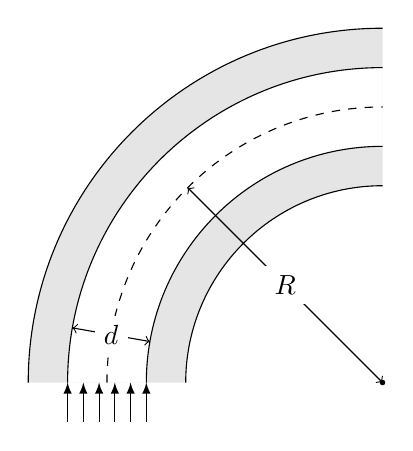
\begin{tikzpicture}    
    \fill[fill=gray!20] (-4.5, 0) arc(180:90:4.5) -- (0, 2.5) arc(90:180:2.5) -- cycle ;
    \draw (-4.5, 0) arc(180:90:4.5) (0, 2.5) arc(90:180:2.5);
    \fill[white] (-4, 0) arc(180:90:4) -- (0, 3) arc(90:180:3) -- cycle;
    \draw (-4, 0) arc(180:90:4);
    \draw (-3, 0) arc(180:90:3);
    \draw[dashed] (-3.5, 0) arc(180:90:3.5);
    \fill (0,0) circle(1pt) coordinate (O);
    \foreach \x in {-4, -3.8,..., -3}{
      \draw[-latex] (\x, -0.5) -- (\x, 0);
    }
    \draw[<->] (O) -- (135:3.5) node[midway, fill=white]{$R$};
    \draw[<->] (170:4) -- (170:3) node[midway, fill=white]{$d$};
  \end{tikzpicture}
\end{document}
